\documentclass{article}
\title{\sc Secador de Aire, Tipo Refrigerado.}
\author{\it Erick I. Rodríguez Juárez.}
\usepackage[margin = 0.5in]{geometry}
\usepackage{graphicx}
\usepackage{amsmath}
\begin{document}
\maketitle

\section{\centering --- Variables ---} % (((
Se definen:
\begin{center}
  \begin{tabular}{|l|l|l|}
    \hline 
    Variable & Descripción   & Unidades\\ \hline 
    Y:  & Precio del activo  & MXN \\ \hline 
    X1: & Edad del activo    & Años \\ \hline 
		X2: & Capacidad & \(hp\) \\ \hline 
  \end{tabular}
\end{center} 
% )))

\section{\centering --- Datos Usados ---} % (((
Se toma una muestra estadísticamente significativa. \\ 
La comprobación de este hecho se realiza la comprobación de este hecho a lo largo de las siguientes secciones.
\begin{center}
	\begin{tabular}{*{4}{|p{3cm}}|}
		\hline 
MARCA          & EDAD  & CAP  & PRECIO\\ \hline
Speedaire      & 0     & 35   & 104750.90\\ \hline
Hankison       & 0     & 25   & 54461.60\\ \hline
Ingersoll Rand & 0     & 15   & 151014.60\\ \hline
Atlas Copco    & 11    & 14   & 31224.75\\ \hline
Beko           & 4     & 50   & 27650.00\\ \hline
Kaeser         & 11    & 20   & 18555.50\\ \hline
Atlas Copco    & 3     & 63   & 28379.00\\ \hline
Atlas Copco    & 18    & 32   & 15701.25\\ \hline
	\end{tabular}
\end{center}
% )))

\section{\centering --- Matriz de Dispersion ---} % (((
\begin{center}
  \begin{tabular}{|p{11cm}|p{5cm}|}
    \hline
    Gráfica & Interpretación. \\ \hline 
    \begin{minipage}{\textwidth}
    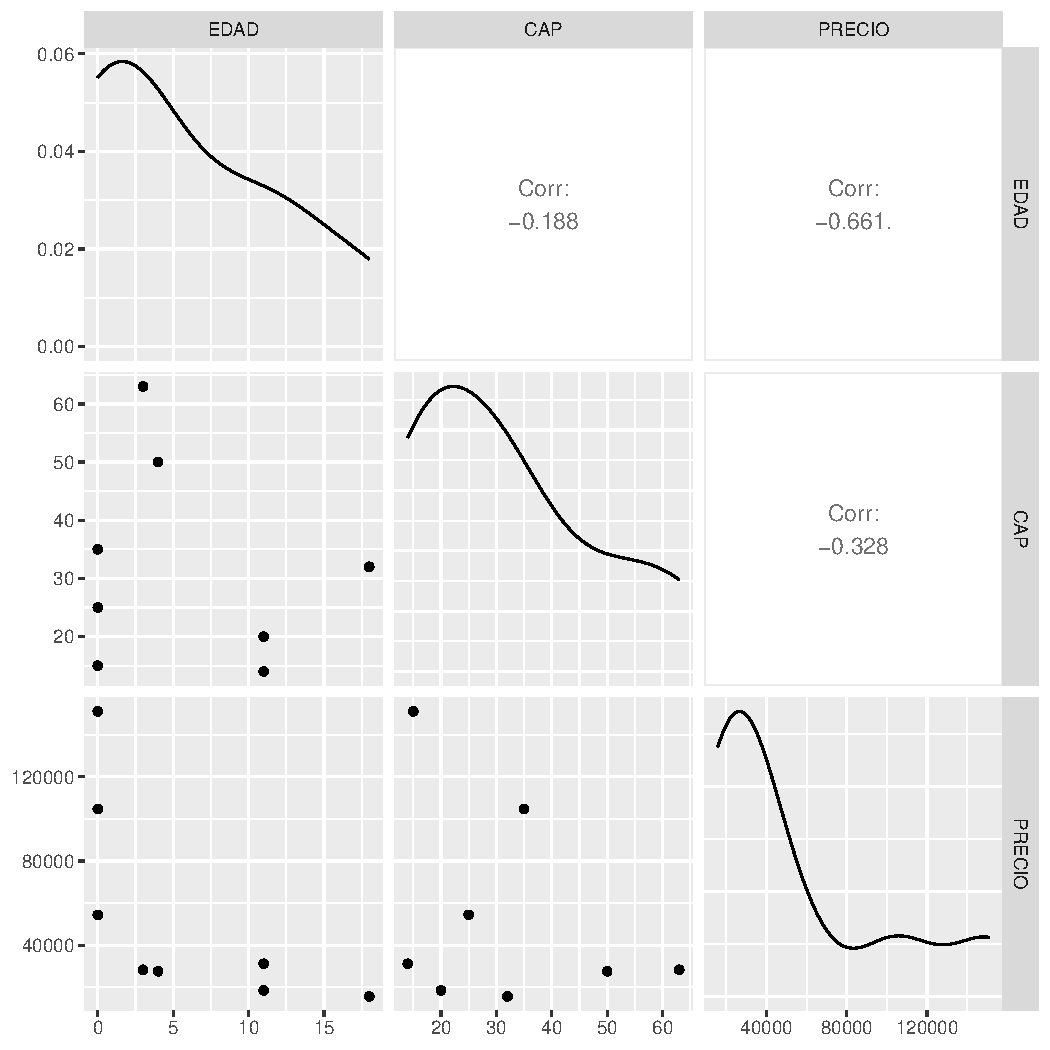
\includegraphics[width= 0.5 \linewidth, page=1]{r/Rplots.pdf}
    \end{minipage} 
    &
		Hay una correlación lineal débil (el \(66.1\%\) de los datos lo confirman),
		entre la Edad y el Precio del activo.
		\\ \hline 
  \end{tabular}
\end{center} 
% )))

\newpage

\section{\centering --- Supuestos del Modelo de Regresión ---} % (((

Se realizará el análisis estadístico con un \(90\%\) de confianza. \\ 
Es decir, \(1- \alpha = 0.9\).

\subsection{--- Homocedasticidad ---} % (((
\begin{center}
  \begin{tabular}{|l|p{8cm}|}
    \cline{1-2}
    \multicolumn{2}{|c|}{Hipótesis}\\ \cline{1-2}
    \multicolumn{2}{|l|}{\(H_0:\) La varianza de los residuales es constante.} \\ 
    \multicolumn{2}{|l|}{\(H_a:\) La varianza de los residuales no es constante.} \\ \cline{1-2}
    Estadístico de Prueba & \(BP = 4.4606\).\\ \cline{1-2} 
		Región de Rechazo de \(H_0\) & \((0, \alpha )\).\\ \cline{1-2} 
    Valor \(p\) & \(0.1075\).\\ \cline{1-2} 
    Conclusión & Se tiene que \(p> \alpha\). \newline 
		Por tanto no se rechaza \(H_0\). \newline 
		Es decir, la varianza no es constante. \\ \cline{1-2} 
  \end{tabular}
\end{center}
% )))

\subsection{--- Independencia ---} % (((
\begin{center}
  \begin{tabular}{|l|p{8cm}|}
    \cline{1-2}
    \multicolumn{2}{|c|}{Hipótesis}\\ \cline{1-2}
    \multicolumn{2}{|l|}{\(H_0:\) Los residuos son independientes.} \\ 
    \multicolumn{2}{|l|}{\(H_a:\) Los residuos no son indpendientes.} \\ \cline{1-2}
    Estadístico de Prueba & \(DW = 2.7842\).\\ \cline{1-2} 
		Región de Rechazo de \(H_0\) & \((0, \alpha )\).\\ \cline{1-2} 
    Valor \(p\) & \(0.9005\).\\ \cline{1-2} 
    Conclusión & Se tiene que \(p> \alpha\). \newline 
		Por tanto no se rechaza \(H_0\). \newline 
		Es decir, los residuos son independientes.\\ \cline{1-2} 
  \end{tabular}
\end{center}
% )))

\subsection{--- Normalidad ---} % (((
\begin{center}
  \begin{tabular}{|l|p{8cm}|}
    \cline{1-2}
    \multicolumn{2}{|c|}{Hipótesis}\\ \cline{1-2}
    \multicolumn{2}{|l|}{\(H_0:\) Los residuos siguen una distribución normal} \\ 
    \multicolumn{2}{|l|}{\(H_a:\) Los residuos no siguen una distribución normal.} \\ \cline{1-2}
    Estadístico de Prueba & \(W = 0.95507\).\\ \cline{1-2} 
		Región de Rechazo de \(H_0\) & \((0, \alpha )\).\\ \cline{1-2} 
    Valor \(p\) & \(0.7621\).\\ \cline{1-2} 
    Conclusión & Se tiene que \(p> \alpha\). \newline 
		Por tanto no se rechaza \(H_0\). \newline 
		Es decir, los residuos siguen una distribución normal.\\ \cline{1-2} 
  \end{tabular}
\end{center}
% )))

% )))

\newpage

\section{\centering Modelo de Regresión Estimado ---} % (((
\begin{align}
	Y & = &              127,764 & - 5,439 \cdot X_1           & - 1,318     \cdot X_2   \\[2mm]
	\mbox{Precio} & = &  127,764 & - 5,439 \cdot (\mbox{Edad}) & - 1,318     \cdot (\mbox{hp})
	\label{eq:1}
\end{align}
% )))

\section{\centering --- Tabla Anova ---} % (((
\begin{center}
  \begin{tabular}{|l|l|l|l|l|}
    \hline 
    Fuentes de Variación  & Suma de Cuadrados & Grados de Libertad & Cuadrados Medios & F\\ \hline 
Regresión  & 10763470574          &  2       & 5381735287 & 4.62603\\ \hline
Error      &  5816797343          &  5       & 1163359469 & 0.00000\\ \hline
Totales    & 16580267917          &  7       & 6545094756 & 0.00000\\ \hline
  \end{tabular}
\end{center} 
% )))

\section{\centering --- Prueba de Significancia del Modelo ---} % (((
Se comprueba la significancia del modelo con el estadístico \(F\) de la Tabla Anova.
\begin{center}
  \begin{tabular}{|l|p{6cm}|}
    \cline{1-2}
    \multicolumn{2}{|c|}{Hipótesis}\\ \cline{1-2}
    \multicolumn{2}{|l|}{\(H_0:\) El modelo no es significativo.} \\ 
    \multicolumn{2}{|l|}{\(H_a:\) El modelo es significativo.} \\ \cline{1-2}
    Estadístico de Prueba & \(4.626\).\\ \cline{1-2} 
		Región de Rechazo de \(H_0\) & \((0, \alpha )\).\\ \cline{1-2} 
    Valor \(p\) & \(0.0729\).\\ \cline{1-2} 
    Conclusión & Se tiene que \(p<\alpha\). \newline 
		Por tanto se rechaza \(H_0\). \newline 
		Es decir, el modelo es significativo.\\ \cline{1-2} 
  \end{tabular}
\end{center} 
% )))

\section{\centering Estimación del Valor de Mercado aplicado al Activo.} % (((
Se obtiene el valor de mercado por medio de las características del activo y el modelo de regresión \eqref{eq:1}.
\begin{center}
  \begin{tabular}{|l|l|l|}
    \hline 
		Descripción   & Unidades  & Activo \\ \hline 
    Edad del activo    & Años      & 2      \\ \hline 
		Capacidad  & \(hp\) & 35   \\ \hline 
		Precio del activo   & MXN       & \$59,786.41   \\ \hline 
  \end{tabular}
\end{center} 
% )))

\end{document}
